\section{Reference Profile Comparison}

The comparison below is illustrative, policy-weighted, and non-normative. The standard is the merge witness and conformance artifact boundary, not a stack ranking. The scores assume durable product systems with web product surface, API/service behavior, operational security requirements, and long-running maintenance by agents and humans together. Alternative stacks can conform when they produce equivalent proof receipts and merge witnesses.

\begin{table}[t]
\caption{Reference profile results under the jankurai scoring model.}
\label{tab:stack-ranking}
\centering
\small
\begin{tabularx}{\columnwidth}{L{0.10\columnwidth} Y L{0.13\columnwidth}}
\toprule
\textbf{Rank} & \textbf{Stack} & \textbf{ANSS} \\
\midrule
1 & Rust core + TypeScript/React/Vite + PostgreSQL & 94 \\
2 & Go services + TypeScript/React/Vite + PostgreSQL & 90 \\
3 & C\#/.NET + TypeScript/React/Vite + PostgreSQL & 89 \\
4 & TypeScript product plane + Rust/Go compute cells + PostgreSQL & 88 \\
5 & Kotlin/Java JVM + TypeScript/React/Vite + PostgreSQL & 87 \\
\bottomrule
\end{tabularx}
\end{table}

\begin{figure*}[t]
\centering
\IfFileExists{paper/figures/stack-ranking.pdf}{%
  \includegraphics[width=0.94\textwidth]{paper/figures/stack-ranking.pdf}%
}{%
  \includegraphics[width=0.94\textwidth]{figures/stack-ranking.pdf}%
}
\vspace{-0.4em}
\caption{Reference profile comparison by Agent-Native Stack Score (ANSS), the weighted jankurai scoring model. The figure is a zoomed comparison of close contenders; Table~\ref{tab:stack-ranking} gives the policy scores. Labels: RUST = Rust core, GOSV = Go services, NET = C\#/.NET, TSRG = TypeScript product plane with Rust/Go compute cells, and JVM = Kotlin/Java. All entries assume TypeScript/React/Vite product surface and PostgreSQL durable truth; streaming buses are workload-specific additions.}
\label{fig:stack-ranking}
\end{figure*}

\begin{table*}[t]
\caption{Representative score decomposition. Bands express policy uncertainty, not statistical confidence.}
\label{tab:score-decomposition}
\centering
\scriptsize
\begin{tabularx}{\textwidth}{L{0.24\textwidth} L{0.08\textwidth} L{0.08\textwidth} L{0.08\textwidth} L{0.08\textwidth} L{0.08\textwidth} L{0.08\textwidth} Y}
\toprule
\textbf{Stack family} & \textbf{Proof} & \textbf{Sec.} & \textbf{Runtime} & \textbf{Boundary} & \textbf{Ops} & \textbf{Band} & \textbf{Exception logic} \\
\midrule
Rust + TS/Vite + Postgres & 18 & 16 & 13 & 11 & 36 & $\pm 3$ & Default when no stronger domain constraint exists. \\
Go + TS/Vite + Postgres & 16 & 13 & 13 & 10 & 38 & $\pm 4$ & Strong cloud-service default where simplicity beats type-state power. \\
.NET + TS/Vite + Postgres & 16 & 13 & 12 & 10 & 38 & $\pm 4$ & Strong regulated enterprise answer when Microsoft platform fit speeds proof. \\
Full-stack Next.js + Postgres & 13 & 10 & 9 & 8 & 36 & $\pm 6$ & Excellent product loop; needs stricter backend/data partitioning to avoid truth drift. \\
Python/FastAPI + Postgres & 10 & 8 & 8 & 7 & 34 & $\pm 7$ & Useful AI/data boundary; risky as durable product core. \\
Rails + Postgres & 11 & 9 & 8 & 7 & 36 & $\pm 6$ & Fast CRUD app fit; needs generated contracts and stronger service boundaries. \\
Elixir/Phoenix + Postgres & 14 & 11 & 11 & 8 & 37 & $\pm 5$ & Specialist override for realtime collaboration and supervision-heavy systems. \\
JVM/Spring or Kotlin + Postgres & 15 & 11 & 11 & 10 & 40 & $\pm 5$ & Brownfield and enterprise fit can outweigh default-stack migration cost. \\
\bottomrule
\end{tabularx}
\end{table*}

Sensitivity is concentrated in three weights: memory safety/security, ecosystem corpus strength, and runtime/concurrency. Increase ecosystem weight and Go, .NET, and JVM improve. Increase type-state and memory-safety weight and Rust separates. Increase product velocity and full-stack TypeScript rises, but it hits hard filters unless durable truth, generated contracts, and server ownership are explicit. These scores are reproducible from stated assumptions, not empirical universals.

\subsection{Streaming Infrastructure: Kafka Today, Rust Tomorrow}

Kafka deserves separate treatment because it is both proven and not the baseline. It remains a high bar for durable distributed streaming: it combines replicated logs, high availability, Connect, Streams, client depth, production operating knowledge, and exactly-once processing semantics in the Streams ecosystem \cite{kafkaIntro2026,kafkaStreams2026,kafkaRebalance2026}. The jankurai position is explicit: Kafka is a brownfield exception, not stack identity. Use it when the system already needs it, isolate it behind generated event contracts and observable Rust queue adapters, and keep the replacement question measurable.

\begin{table*}[t]
\caption{Rust-facing streaming candidates for an agent-native stack.}
\label{tab:streaming-candidates}
\centering
\scriptsize
\begin{tabularx}{\textwidth}{L{0.16\textwidth} Y Y}
\toprule
\textbf{Runtime} & \textbf{Strength} & \textbf{Agent-native caution} \\
\midrule
Kafka & Proven baseline for distributed event streaming, Connect, Streams, client ecosystem, HA, and production operations. & JVM and operations gravity are real; keep it behind adapters rather than letting it define the stack. \\
Tansu & Strongest Kafka-compatible Rust candidate to watch: stateless broker, Kafka API, PostgreSQL/S3/SQLite storage, schema-backed topics, and Iceberg/Delta/Parquet paths \cite{tansuGithub2026,tansuInfoQ2026}. & Not yet a default replacement; ACLs/throttling and S3 compaction/deletion remain explicit gaps in public coverage \cite{tansuInfoQ2026}. \\
Apache Iggy & Strong Apache/Rust-native streaming platform with persistent streams, low latency goals, SDKs, and S3-compatible backup \cite{apacheIggy2026}. & Greenfield Rust-native option, not a Kafka-wire-compatible drop-in. \\
Fluvio & Rust/WASM streaming platform positioned as Kafka plus Flink-style processing in one product \cite{fluvio2026}. & Compelling greenfield alternative, not a brownfield Kafka replacement by protocol. \\
RobustMQ & Ambitious Rust multi-protocol messaging project with Kafka protocol work underway \cite{robustmqKafka2026}. & Kafka support is still incomplete; treat as evaluation material, not replacement proof. \\
\bottomrule
\end{tabularx}
\end{table*}

The roadmap for Rust Kafka-class maturity is therefore a proof program, not a slogan: protocol contract and client golden tests; single-broker produce/fetch; durable log and crash recovery; consumer groups and offsets; replication, controller behavior, and leader epochs; retention and compaction; transactions, security, ACLs, and quotas; then operations, observability, migration tools, and chaos tests. The benefit is not fashion. It is escaping JVM runtime surface where possible, reducing memory and operations cost, preserving Rust-first safety, and giving agents fewer divergent runtime models to reason about.
